\begin{multicols}{3}Останахме хора, които се обичат и подкрепят
\byline{Третият випуск}{Митрушка Славова, випуск 1967г. бивш зам. директор на гимназията}
Третият випуск на НЕГ "Вилхелм Пик" - 1962- 1967 е също част от историята на училището. Тогава, когато се пързаляхме по пантофи на последния етаж на Мъжката гимназия/ Гълъбарника/ и всеки имаше шкафче за учебниците си в училище, всички бяхме задължително на занималня до 10 клас, успяхме и се доказахме без изключение! 
Имахме прекрасни учители, от които се учехме, копирахме доста неща, 
имаше кръжоци на свещи, всяка събота - забава в еврейския дом/сега Картинна галерия/, покорявахме върхове, участвахме в бригади. Но най-същественото е, че си останахме хора, които се обичат и подкрепят... \\[19cm]

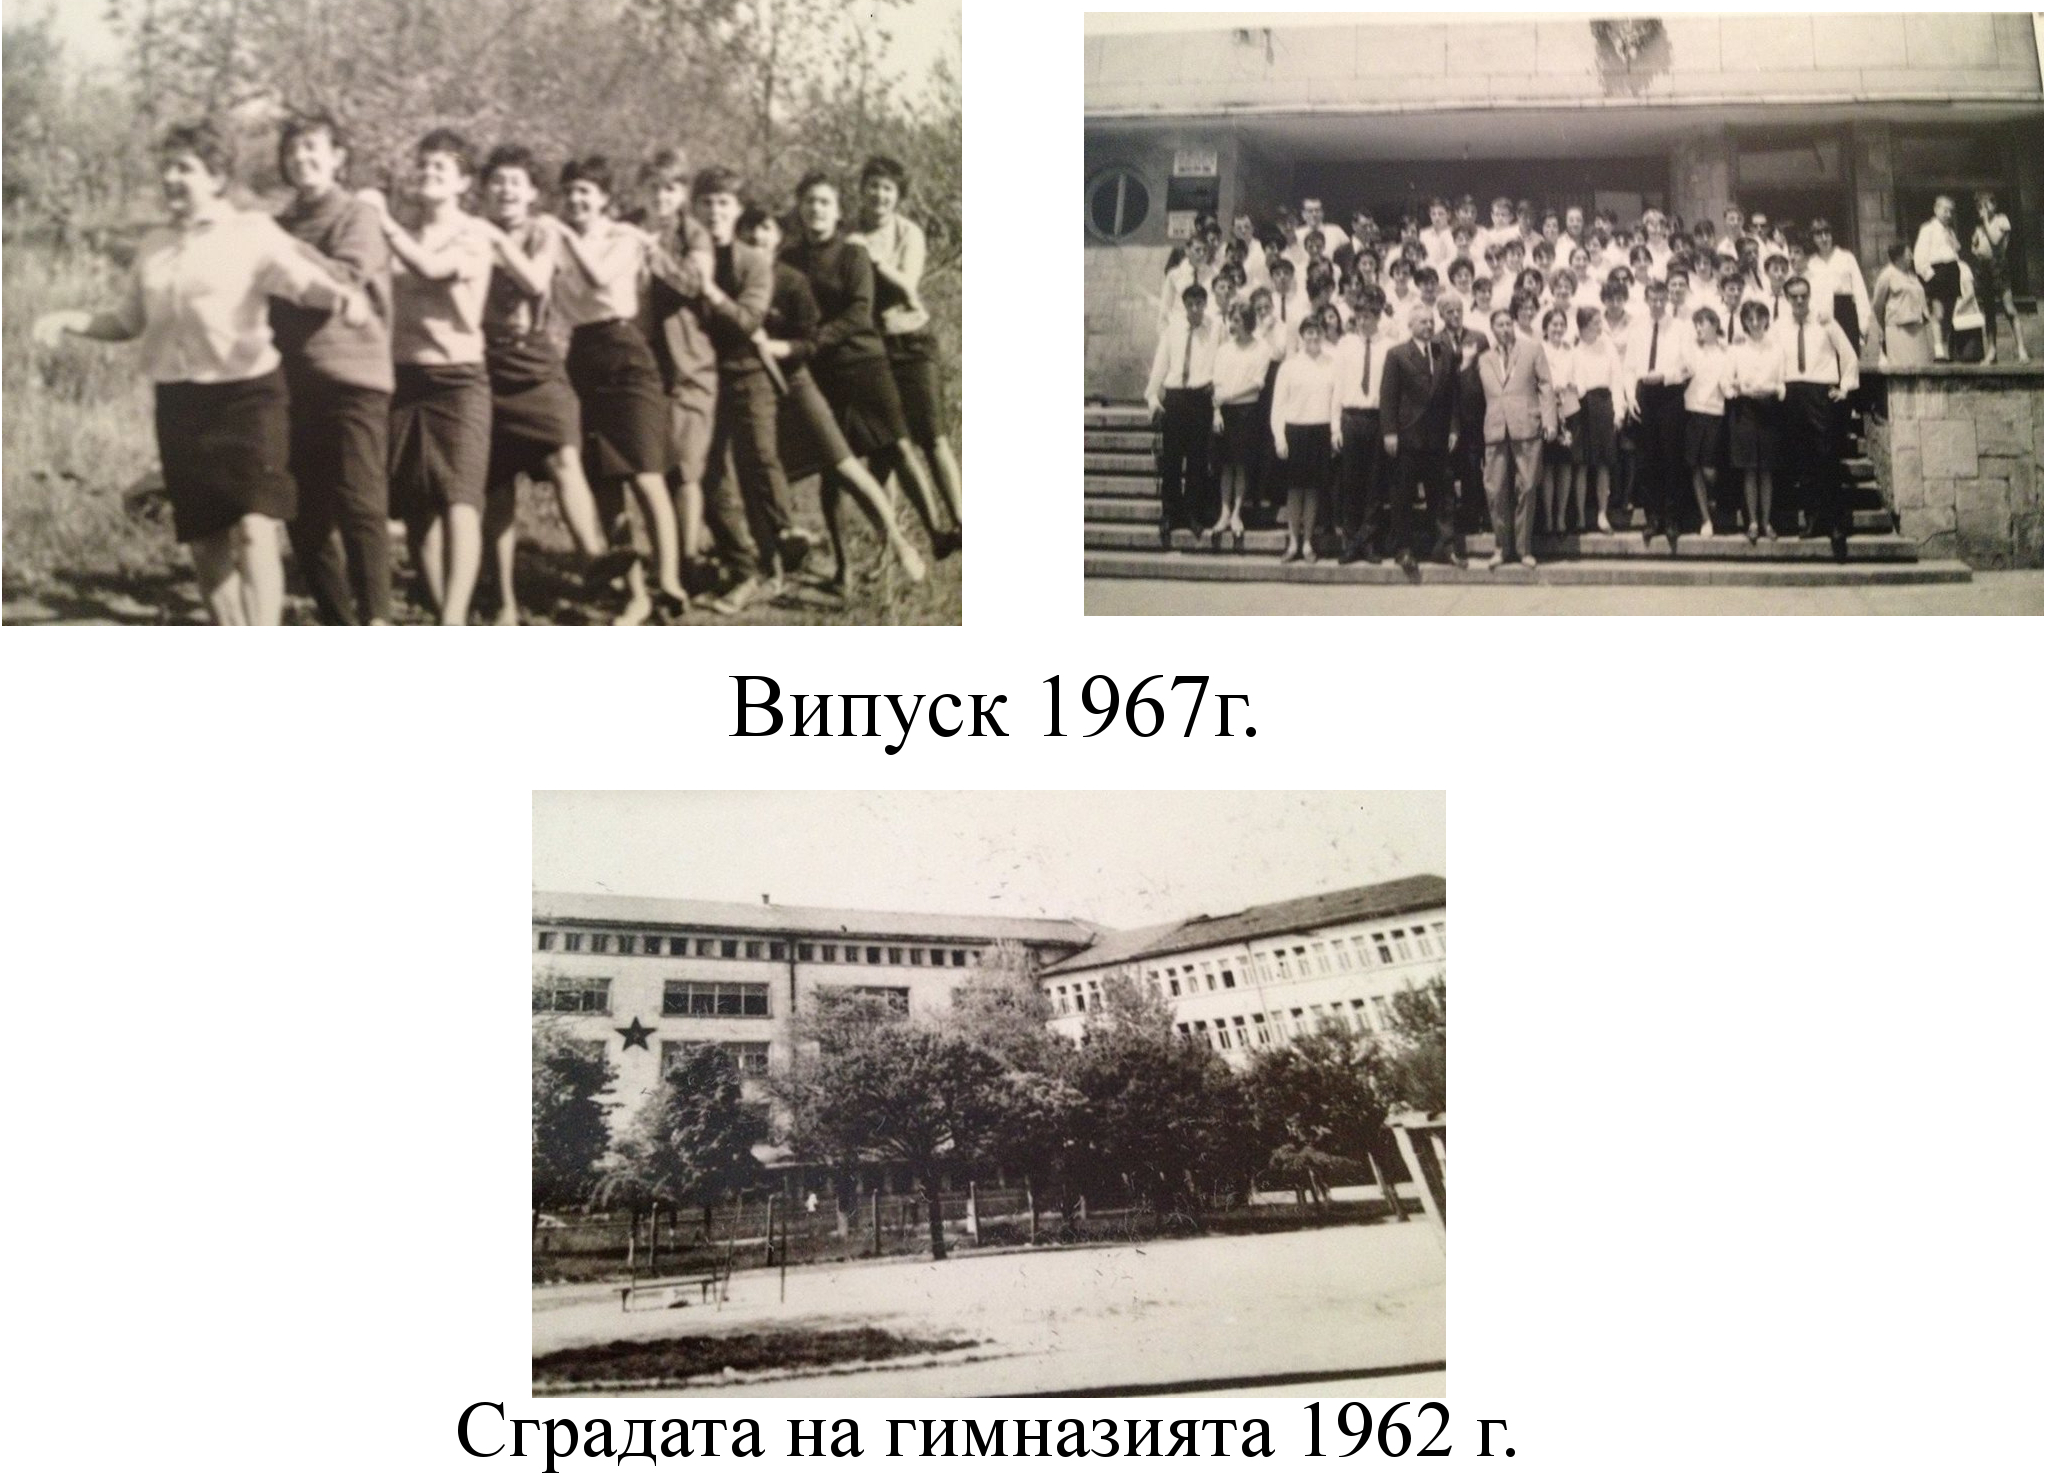
\includegraphics[width=5.5in]{./treti_vipusk/3.jpg} 

% \closearticle
\end{multicols}
